\section{Tracking with the Inner Detector} \label{sec:atlas:tracking}

The Inner Detector (ID), shown in \Cref{fig:inner_detector_diagram}, is
responsible for providing precise momentum resolution and identification of
both primary and secondary vertex measurements of charged particle tracks
\cite{ATLAS-TDR-4,ATLAS-TDR-5}.  The ID's innermost subsystem, the Insertable
B-Layer (IBL), is only $3.3~\cm$ from the interaction point
\cite{Potamianos:2209070} and thus must be able to perform its crucial duties
while enduring the high fluence of radiation from the colliding beams.

\begin{figure}[!htbp]
  \begin{center}
    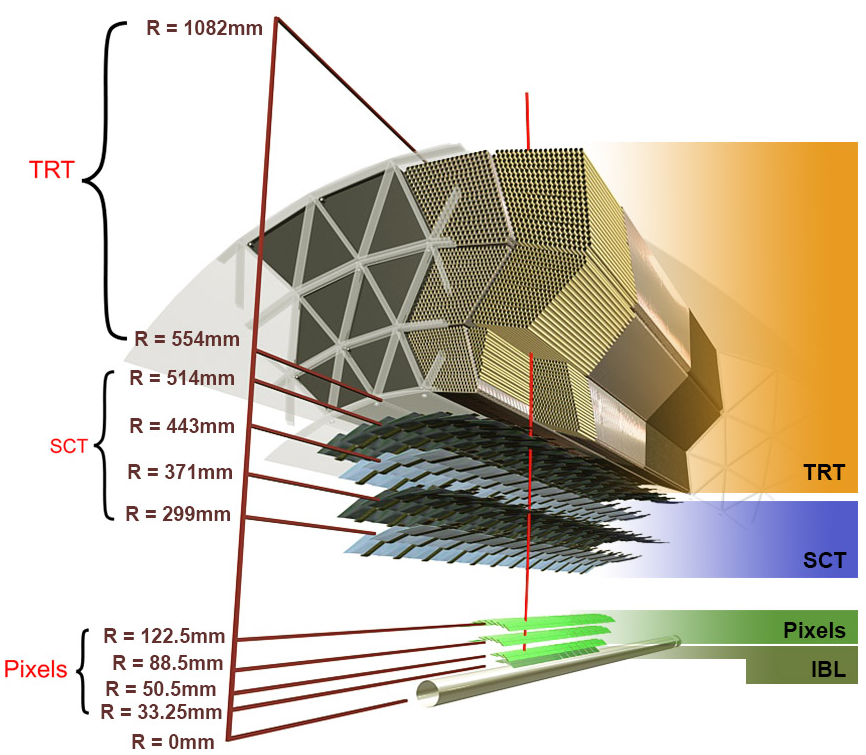
\includegraphics[width=0.8\linewidth]{figures/atlas/inner_detector_diagram}
    \caption{Diagram of inner detector \cite{Potamianos:2209070}.}
    \label{fig:inner_detector_diagram}
  \end{center}
\end{figure}

The ID is designed to be very compact to reduce the probability of a particle
decaying inside and to give precision measurements of the particles' curvature in
the 2 T solenoidal magnetic field. This leads to excellent momentum resolution
above the nominal \pT threshold of $0.5~\GeV$ and within the pseudorapidity range
of $|\eta| < 2.5$ as shown in \Cref{fig:inner_detector_schematic}.

\begin{figure}[!htbp]
  \begin{center}
    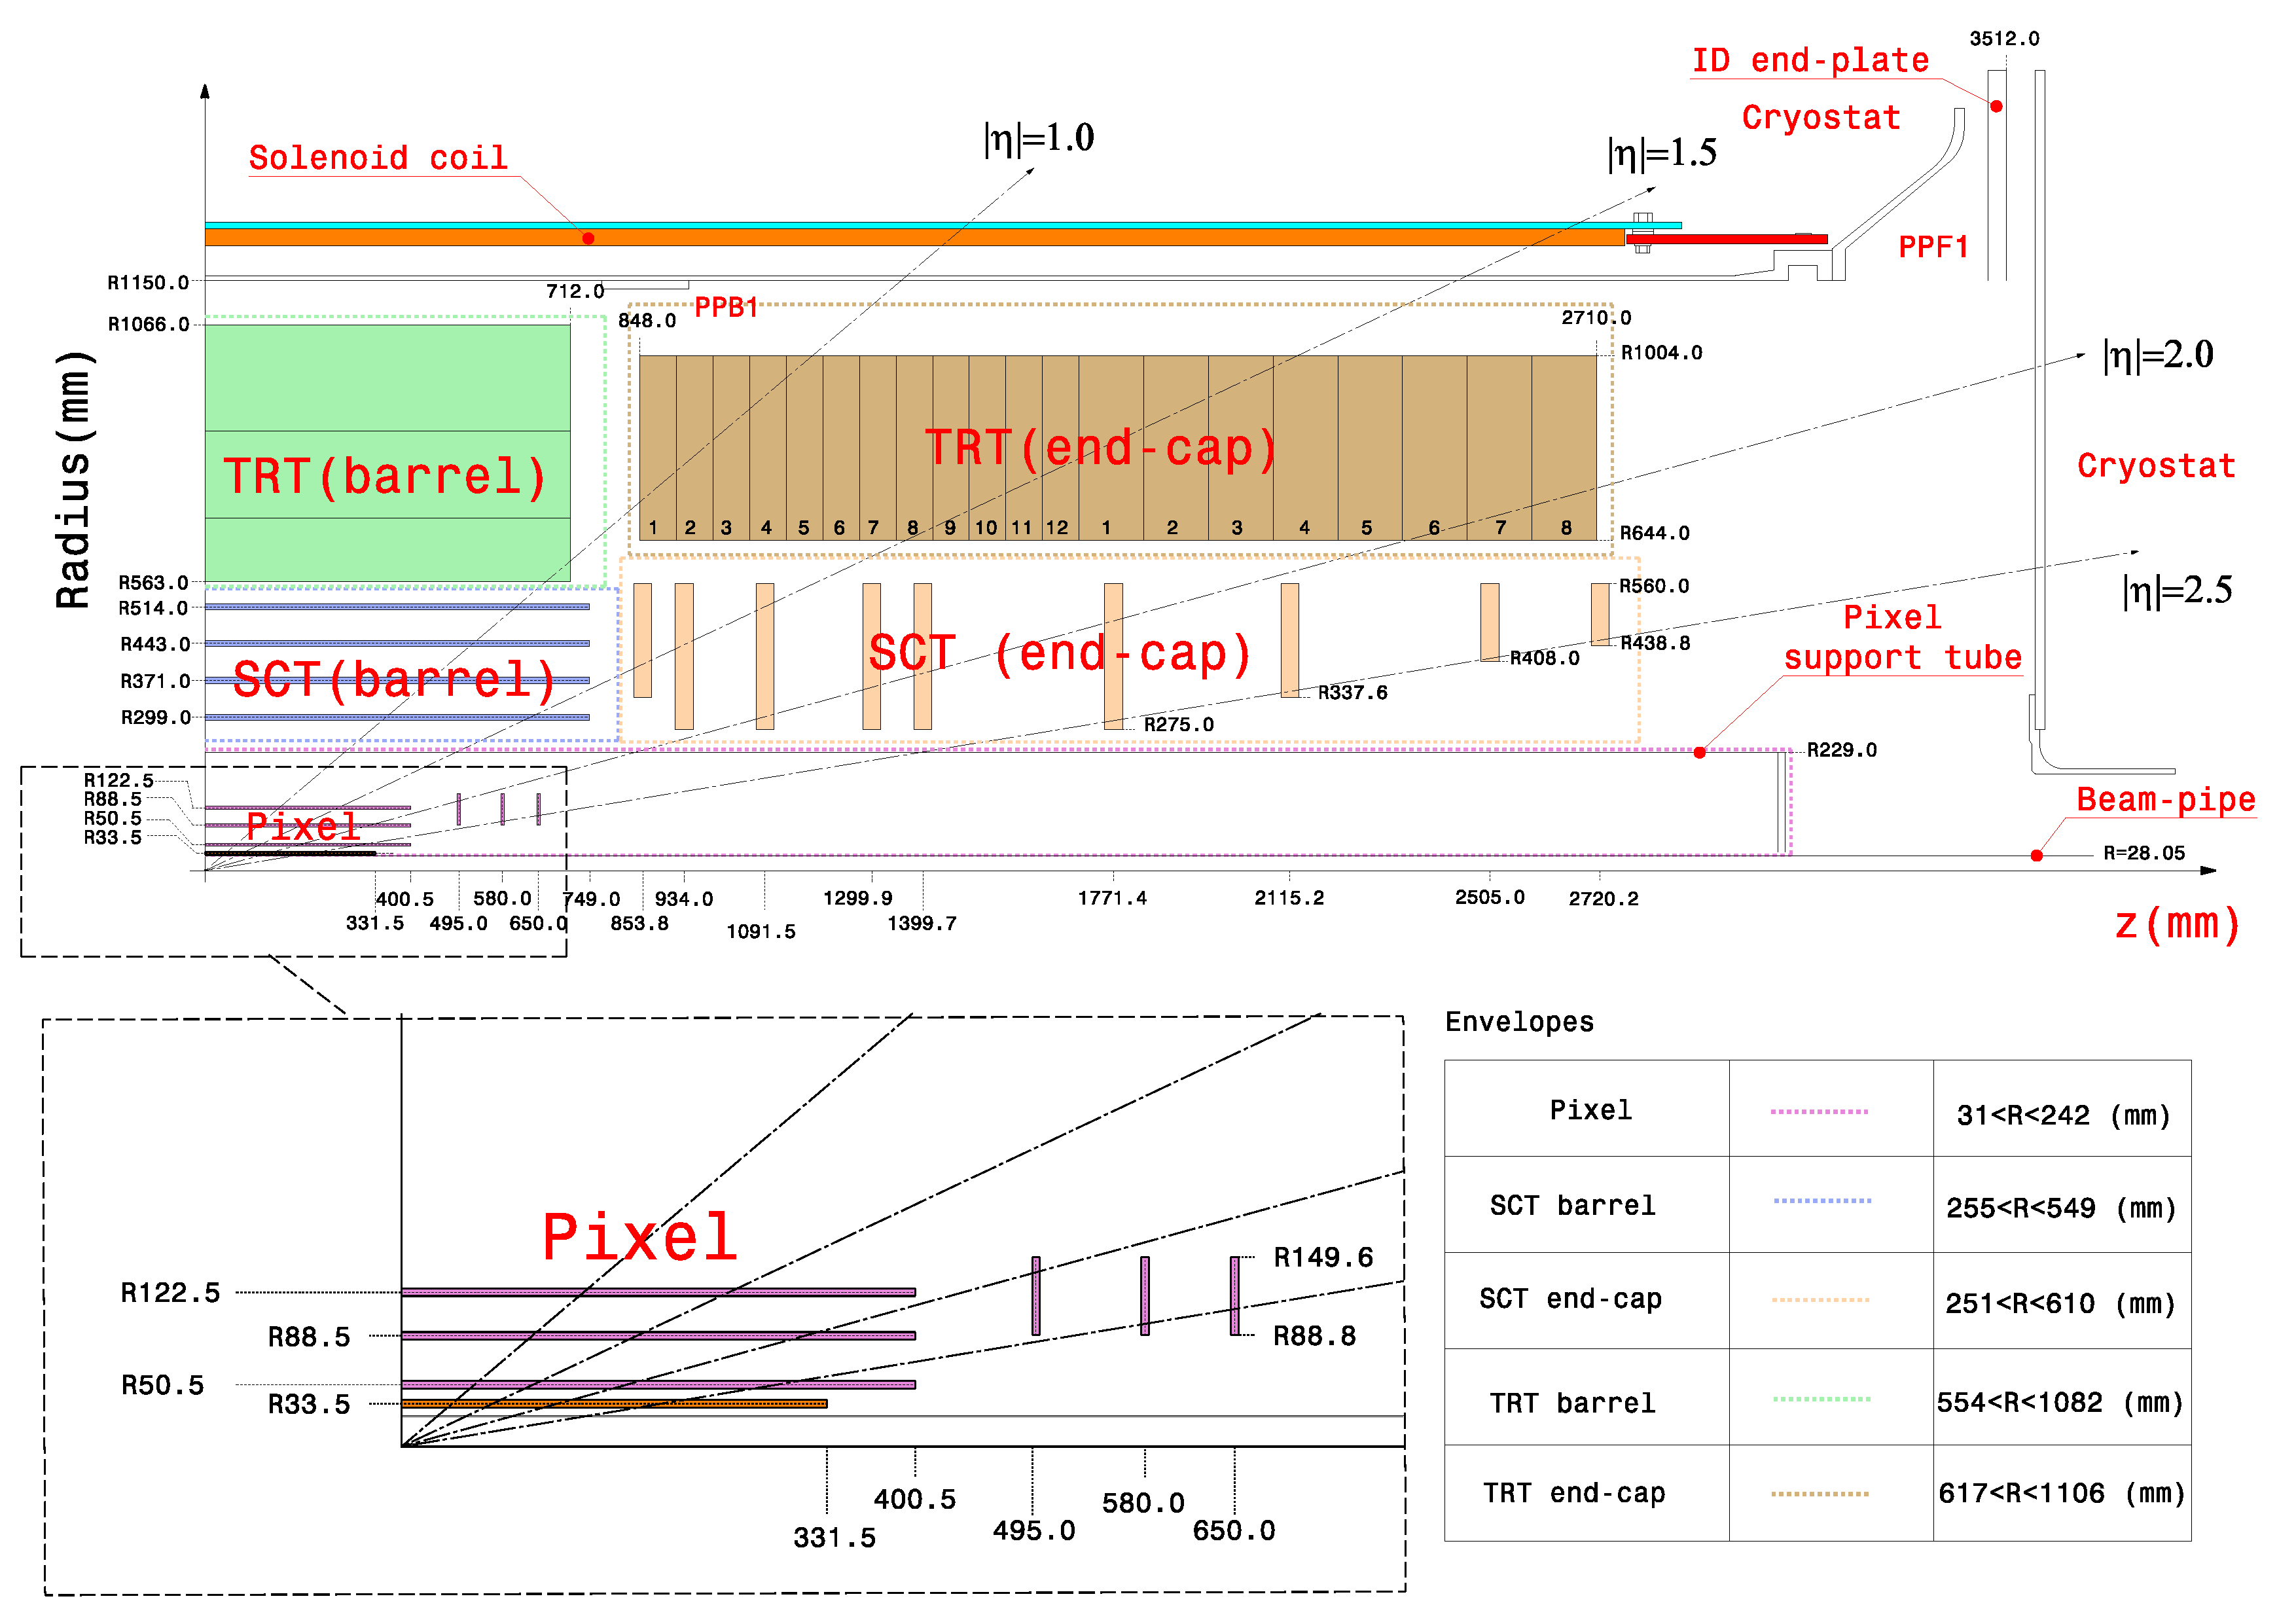
\includegraphics[width=0.8\linewidth]{figures/atlas/inner_detector_schematic}
    \caption{Schematic of the Inner Detector including $\eta$
lines.  Each component shown is cylindrically symmetric leading to a
multi-layered detector \cite{PIX-2018-001}.}
    \label{fig:inner_detector_schematic}
  \end{center}
\end{figure}

The ID is composed of three different detector technologies for particle
trajectory reconstruction: Pixel Detector (including the IBL), Semiconductor Tracker (SCT) and
the Transition Radiation Tracker (TRT).  These will be discussed in the
following sections. 

\subsection{Pixel Detector}

The ATLAS Pixel Detector \cite{PERF-2007-01}, the innermost subdetector of the ID, is designed to
give the best resolution possible as close as possible to the interaction point.
This is accomplished using the 4 barrel layers and 3 disks per end-cap as
indicated in \Cref{fig:inner_detector_schematic}. The innermost barrel
layer, the IBL, has pixel dimensions of $50~\micm(\hat{\phi}) \times 250~\micm
(\hat{z}) \times 200~\micm (\hat{r})$.  For the other layers the dimensions are
$50~\micm (\hat{\phi}) \times 400 ~\micm (\hat{z})$ for about $90\%$ of the pixels
and $50 ~\micm (\hat{\phi}) \times 600 ~\micm (\hat{z})$ for the others, all with a
thickness of $250 ~\micm (\hat{r})$.  This gives a total active area of $1.88~\meter^2$
collected through 92.4 million readout channels, more than half of the total
number of channels for ATLAS. This detailed charged particle information very
close to the interaction point is crucial not only for pattern recognition and
track reconstruction, but also for the reconstruction of the primary and
secondary vertices intrinsic to the decay of $b$-hadrons, a critical element
of the analysis presented in this thesis.

\subsection{Semiconductor Tracker}

Surrounding the Pixel Detector, the Semiconductor Tracker (SCT)
\cite{PERF-2007-01} is composed of 4088 double-sided silicon microstrip modules.
Each side of a module is constructed out of two silicon strip sensors
that are daisy-chained together.  The result is 768 composite strips each
$12.6~\cm$ long with an inter-strip pitch of $80~\micm$. In the barrel the
strips are aligned with the $\hat{z}$ direction, while in the end-caps they are
aligned with the $\hat{r}$ direction. In both cases the separation of the
strips is constant in $\hat{\phi}$. The two sides are rotated with respect to
each other by $40~\text{mrad}$ to allow for position measurement along the
length of the strip.  These modules are then used to tile the 4 barrel layers
and 9 disks per end-cap (18 disks in total) as seen in
\Cref{fig:inner_detector_schematic}.  This design is chosen to ensure that each
charged track interacts with 8 strip layers (equivalent to four space points).
This information is used to further measure the momentum and impact parameter
and to identify the vertices of charged particles.

\subsection{Transition Radiation Tracker}

The Transition Radiation Tracker (TRT) \cite{PERF-2007-01}, the outermost
subdetector of the ID, provides tracking information by detecting the
ionization of gas caused by charged particles in $\eta < 2.0$ as they pass
through the 350,000 drift tube channels also known as straws.  The $4~\mm$
diameter straws are filled with a $70\%$ Xe, $27\%$ CO$_2$, and $3\%$ O$_2$ gas
mixture~\footnote{During Run 2 straws belonging to modules with large gas leaks
were filled with a mixture of $70\%$ Ar, $27\%$ CO$_2$, and $3\%$ O$_2$.  Ar is
less efficient at absorbing transition radiation but maintains similar tracking
capabilities as Xe \cite{Aaboud:2017odu}.} and a $31~\micm$ diameter
gold-plated tungsten wire anode at the center for the collection of the
ionization signal.  In the barrel, 73 azimuthally symmetric layers of $144~\cm$
straws are oriented parallel to the beam pipe with an electrical division in
the center of each allowing the two sides to be read out separately.  For each
end-cap the straws are radially oriented in 160 symmetric planes each containing
768 $37~\cm$-long drift tubes shown in \Cref{fig:inner_detector_schematic}.
There are typically 36 TRT ionization hits per charged particle track. 

The TRT also provides electron identification functionality through the
detection of transition radiation.  In both the barrel and the end-caps,
polypropylene fibers (barrel) or foils (end-caps) function as the transition
radiation material which causes the relativistic charged particles to radiate
and thus ionize the gas in the straw.  The amount of transition radiation
produced is proportional to the Lorentz factor meaning that lighter particles
(e.g. electrons) will produce more radiation.  Thus, by defining a high and low
threshold, tracks belonging to electrons can be identified by requiring a
larger fraction of the TRT hits along the track to pass the high threshold.
